\documentclass{beamer}
\usepackage[french]{babel}
\usepackage{hyperref}
\definecolor{links}{HTML}{2A1B81}
\hypersetup{colorlinks,linkcolor=,urlcolor=links}
\usepackage{graphicx}
\usepackage{amsmath,amssymb}
\usepackage{tabularx}
\usepackage{booktabs}
\usepackage[compatibility=false]{caption}
\usepackage[toc,page]{appendix}
\usepackage{minted}
\usepackage{xspace}

\makeatletter
  \def\beamer@calltheme#1#2#3{%
    \def\beamer@themelist{#2}
    \@for\beamer@themename:=\beamer@themelist\do
    {\usepackage[{#1}]{\beamer@themelocation/#3\beamer@themename}}}

  \def\usefolder#1{
    \def\beamer@themelocation{#1}
  }
  \def\beamer@themelocation{}

\patchcmd{\minted@colorbg}{\noindent}{\medskip\noindent}{}{}
\apptocmd{\endminted@colorbg}{\par\medskip}{}{}
\makeatother

\newcolumntype{Y}{>{\centering\arraybackslash}X}

\usefolder{../theme}
\usetheme[numbering=fraction,block=fill,progressbar=frametitle]{metropolis} %Use metropolis theme

\definecolor{bg}{rgb}{0.95,0.95,0.95}
\setminted{bgcolor=bg,fontsize=\scriptsize,autogobble,mathescape,breaklines,tabsize=2}
\setmintedinline{breaklines,autogobble,fontsize=\scriptsize}
\setbeamersize{text margin left=8pt,text margin right=8pt}
\setbeamercovered{transparent}

\begin{document}

\title[C++]{Introduction à la programmation en C++}
\author[nicolas.audebert@onera.fr]{Nicolas Audebert}
\setmainfont{Fira Sans}


\AtBeginSection[]{
  \begin{frame}{Plan de la séance}
  \small \tableofcontents[currentsection]
  \end{frame}
}

\newcommand\cppi[1]{\mintinline{cpp}{#1}}
\newcommand\cpp[1]{%
  \begin{minted}{cpp}
  #1
  \end{minted}
}%

\author[nicolas.audebert@onera.fr]{Nicolas Audebert}
\date[8 déc. 2017]{Vendredi 8 décembre 2017}
\subtitle{Vecteurs - Templates}
\maketitle

\begin{frame}{Avant toute chose}
  \begin{alertblock}{Rendus de TP et des exercices}
  Les rendus se font sur \href{https://educnet.enpc.fr}{\textbf{Educnet}}, même en cas de retard. \textbf{Pas par mail}.
  \begin{enumerate}
  	\item Le code rendu \textbf{doit compiler}.
    \item Le code rendu doit \textbf{être propre} (indentation, noms de variables clairs).
    \item Le code rendu doit \textbf{être commenté} (réponses aux questions, fonctionnement du code).
    \item Rassembler le code dans une seule archive (\texttt{.zip}, \texttt{.rar}, \texttt{.tar.gz}, etc.).
  \end{enumerate}
  Un exercice ou un TP rendu en retard ou ne respectant pas une des consignes ci-dessus sera pénalisé.
  \end{alertblock}
\end{frame}

\section{STL : vector}

\begin{frame}{STL\,: Standard Template Library}
    \begin{block}{\textbf{S}tandard \textbf{T}emplate \textbf{L}ibrary}
        \begin{itemize}
            \item Bibliothèque de fonctions disponible de base en C++
            \item Elle contient de nombreux modules :
                \begin{itemize}
                    \item Structures de données : chaînes de caractères, tableaux, piles\dots
                    \item Algorithmes classiques : tri, n\up{ième} éléments\dots
                    \item Lecture/écriture (console, fichiers, réseau\dots)
                \end{itemize}
        \end{itemize}
    \end{block}
    \begin{exampleblock}{Quelques exemples}
    Nous avons déjà utilisé la STL, notamment les modules \texttt{iostream} et \texttt{string}.
    \end{exampleblock}
\end{frame}

\begin{frame}[fragile]{Les vecteurs de la STL}
    La STL propose une implémentation de vecteurs dans la classe \texttt{vector}.
    \begin{itemize}
        \item Utilise les tableaux dynamiques
        \item Abstraction de la gestion de la mémoire
        \item Expose une interface type tableau
    \end{itemize}
    
Utilisation\,:
        \begin{minted}{cpp}
#include <vector>

using namespace std;
        \end{minted}
    
\end{frame}

\begin{frame}[fragile]{Classe template}
    La classe \texttt{vector} est une classe template, elle peut s'adapter à tous les types de données. À la compilation, la classe est spécialisée pour le type de données en question.
    
        \begin{minted}{cpp}
// Création d'un vecteur d'éléments de type T
vector<T> tab;

// Exemples :
vector<int> t_int;
vector<double> t_double;
vector<Matrix> t_mat;
vector<float*> t_point;
        \end{minted}
\end{frame}

\begin{frame}[fragile]{Manipulation des vecteurs de la STL}
    Les vecteurs de la STL s'utilisent de la même façon que les tableaux statiques ou dynamiques.
    
        \begin{minted}{cpp}
// Création d'un vecteur d'entiers de 100 éléments
vector<int> t(100);

// L'accès aux cases se fait par l'opérateur []
for(int i=0; i<100; i++){
    t[i] = i*i;
}
cout << t[5] << endl;
		\end{minted}
        
Les vecteurs disposent d'une méthode \texttt{size} permettant de récupérer leur taille\,:
		\begin{minted}{cpp}
cout << t.size() << endl;
        \end{minted}
\end{frame}

\begin{frame}[fragile]{Manipulation des vecteurs de la STL}
    \begin{itemize}
    \item Création et remplissage :
        \begin{minted}{cpp}
// Création d'un vecteur de 100 réels valant tous 5.6
vector<double> t2(1000, 5.6);
        \end{minted}
    \item Redimensionner un vecteur :
    
        \begin{minted}{cpp}
// Création d'un vecteur de 100 éléments de type T
vector<T> t(100);
// Redimensionnement
t.resize(1000);
        \end{minted}
    
    Les éléments déjà existants sont conservés, sauf si la taille finale du vecteur est inférieure à la taille initial, auquel cas les éléments surnuméraires disparaissent.    
    \end{itemize}
\end{frame}

\begin{frame}[fragile]{Manipulation des vecteurs de la STL}
    \begin{itemize}
    \item Accéder au premier élément\,:
    
        \begin{minted}{cpp}
cout << *t.begin() << endl;
        \end{minted}
    
    Il s'agit d'un itérateur, qui fonctionne de manière similaire à un pointeur.
    \item Accéder à la fin du vecteur\,:
    
        \begin{minted}{cpp}
t.end(); // Attention pointe juste derrière la dernière case
        \end{minted}
    \alert{Ce n'est pas le dernier élément !}
    \end{itemize}
\end{frame}

\begin{frame}[fragile]{Manipulation}
    \begin{itemize}
    \item Concaténer deux vecteurs:
    
        \begin{minted}{cpp}
vector<int> t1 (10,2);
vector<int> t2 (30, 100);
t2.insert(t2.end(), t1.begin(), t1.end());
        \end{minted}
    
  	On ajoute le vecteur \texttt{t1} à la fin du vecteur \texttt{t2}.
    \item Trier un vecteur :
    
        \begin{minted}{cpp}
#include <algorithm>

...

std::sort(t.begin(), t.end());
        \end{minted}
    \end{itemize}
\end{frame}

\begin{frame}{TP}

    \begin{minipage}{0.47\linewidth}
        \begin{block}{Serpent}
            Un serpent qui se déplace et s'allonge tout les x pas de temps.
        \end{block}
            \begin{block}{Tron}
                Un serpent deux joueurs qui s'allonge à tout les pas de temps.
            \end{block}

    \end{minipage}
    \hfill
    \begin{minipage}{0.47\linewidth}
        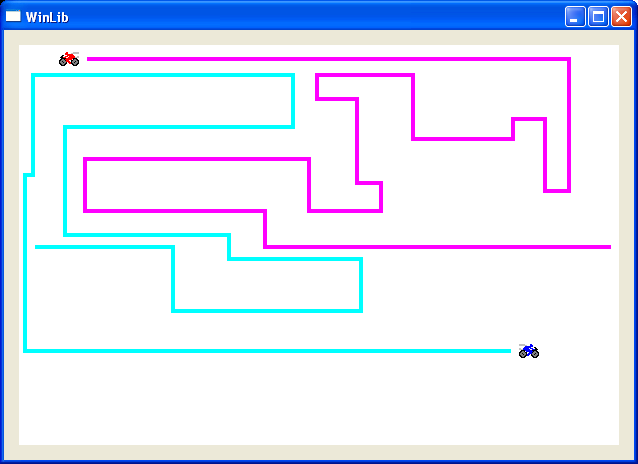
\includegraphics[width=\linewidth]{images/tp.png}
    \end{minipage}
\end{frame}


\end{document}
